\subsubsection{Misaligned Data}


\begin{wrapfigure}[14]{r}{0.5\textwidth}
    \centering
    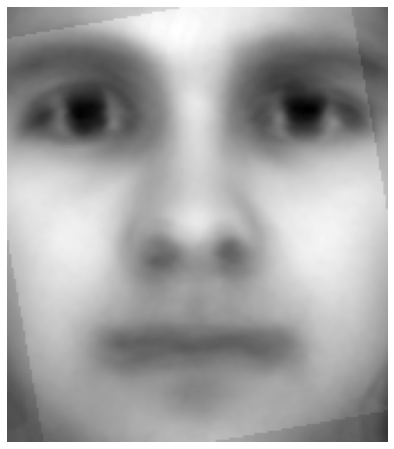
\includegraphics[width=0.9\linewidth]{external_content/media/rotation/average_face-rotation.png}
    \captionsetup{justification=centering}
    \caption{Misaligned eigenface}
    \label{fig:misalignedEigenface}
\end{wrapfigure}

One major problem with \gls{pca} as well as the \gls{svd} is that the units of the data on all axes as well as its alignment significantly impacts the resulting approximation \cite{brunton2019data}.
The demonstration of the eigenfaces solely showcased decent results because the faces have been meticulously centred and cropped manually prior to the evaluation.
The impact can be observed in the adjoining figure \ref{fig:misalignedEigenface}.

To demonstrate the issues, 190 of the 2282 faces have been rotated by 10\textdegree\ prior to the \gls{svd}.
This shows that a mere 8\% is enough to obfuscate the analysis.


% \cite{brunton2019data} (section 1.7)

% \item Showcase Eigenfaces with rotation
% \item only few images ruin the batch
% \item the dataset was meticulously centered and optimized by hand for a proof of concept


\subsubsection{Different units}

\begin{figure}[h]
    \centering
    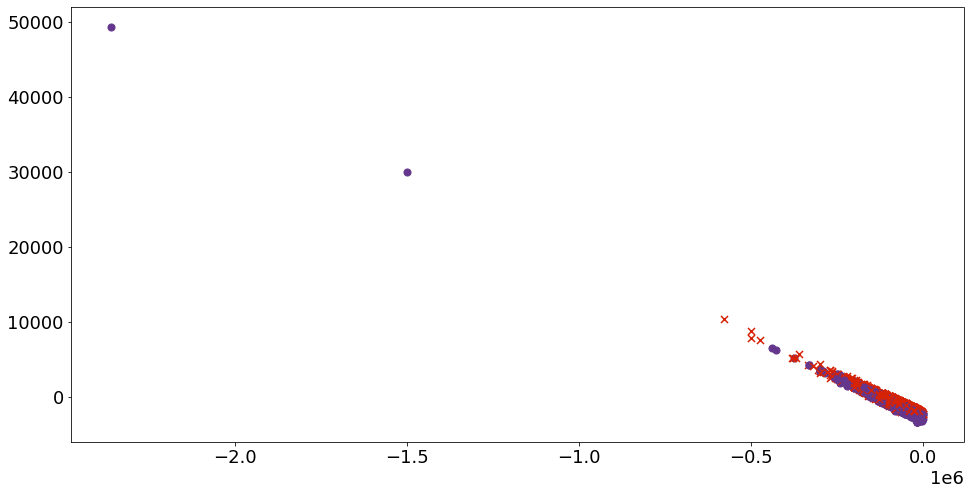
\includegraphics[width=0.8\linewidth]{external_content/media/wrong_units/graph.png}
    \captionsetup{justification=centering}
    \caption{Unit mismatch}
    \label{fig:unitMismatch}
\end{figure}

\noindent
Now we want to showcase what happens when \gls{pca} is applied on a data set with unrelated units.
This examination is based on a \href{https://www.kaggle.com/nehalbirla/vehicle-dataset-from-cardekho?select=Car+details+v3.csv}{vehicle data set} with which we tried to identify patterns in terms of final selling price.
As we can see in figure \ref{fig:unitMismatch}, the graph hardly expresses any useful information.


% Different units WITHIN THE MATRIX... \cite{Jolliffe2002book} (Section 2.3 page 22)

% \item relevant for ALL the values
% \item bigger numbers become dominant no matter what
% \item example car data set. I thought I was being smart... NOPE





\clearpage




\subsubsection{Too broad singular values}

For our last examination we will showcase the effects an adequate choice of \acrlong{pc} has on the resulting evaluation.
We are now considering the Yale Face Database again and comparing two exemplary \glspl{pc} of two people.

\begin{center}
    \begin{figure}[h]
      \centering
      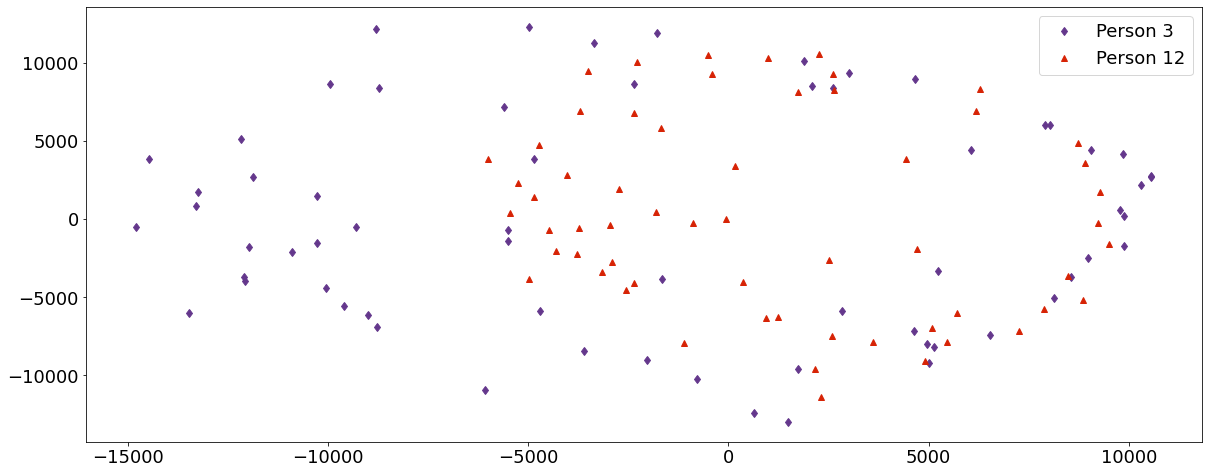
\includegraphics[width=0.9\linewidth]{external_content/media/choice_of_pc/p3_12-pc1_2-centered.png}
      \captionsetup{justification=centering}
      \caption{First two principal components for person 3 and 12}
      \label{fig:pcIandII}
    \end{figure}
\end{center}

\vspace{-8mm}
For the first evaluation in figure \ref{fig:pcIandII} we are considering the two major \glspl{pc} when naively picking the highest singular values.
Each point represents one image from the respective person.
As we can observe, the assertions made from the graph are negligible.
This is due to the \glspl{pc} primarily picking up the biggest similarities in the pictures such as the lighting conditions.

But this does not have to be the end, upon further inspection by trial and error, we can identify \gls{pc} 5 and 6.
Said \gls{pc} propose a split of the graph seen in figure \ref{fig:pcVandVI}.
The values are now noticeably heterogenous and we can make certain observations from their shape.

\begin{center}
    \begin{figure}[h]
      \centering
      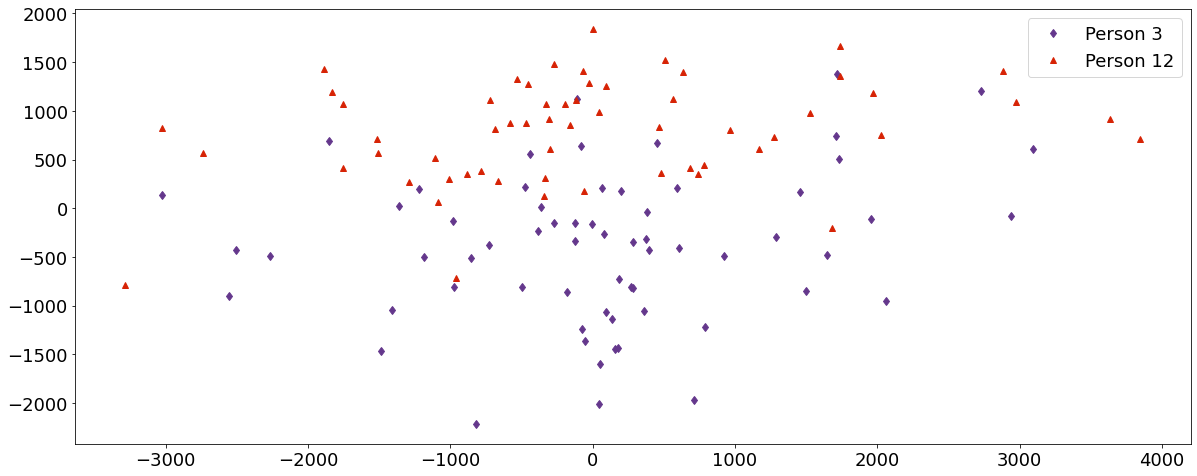
\includegraphics[width=0.9\linewidth]{external_content/media/choice_of_pc/p3_12-pc5_6-centered.png}
      \captionsetup{justification=centering}
      \caption{\gls{pc} 5 and 6 for person 3 and 12}
      \label{fig:pcVandVI}
    \end{figure}
\end{center}

% First principal components might be too general and not \cite{brunton2019data} (section 1.6 - last figure)

% \item Showcase Eigenfaces distribution of the images
% \item 5 and 6 work great
% \item others ruin all the information
% \item all the vertices are one picture of a person
% \item taken with various facial expressions and very different lighting settings

\clearpage
